
% !TEX program = pdflatex
% !TEX enableSynctex = true
% !BIB program = bibtex


\documentclass[12pt]{article}

\usepackage{setspace}
\usepackage{amsmath}
\usepackage{amsfonts}
\usepackage{graphicx}
\usepackage{float}
\addtolength{\oddsidemargin}{-.7in}
\addtolength{\evensidemargin}{-.7in}
\addtolength{\textwidth}{1.4in}
\usepackage{enumerate}
\onehalfspacing
\usepackage{geometry} % Required for customizing page layout

\usepackage{caption}
\usepackage{booktabs}

\usepackage{hyperref}
\hypersetup{
	pdfstartview = FitH,
	pdfauthor = {...},
	pdftitle = {...},
	pdfkeywords = {...; ...; ...; ...},
	colorlinks = true,
	linkcolor = blue,
	urlcolor = blue,
	citecolor = blue,
	linktocpage=true
}


\DeclareMathOperator{\E}{\mathbb{E}}
\DeclareMathOperator*{\argmax}{arg\,max}
\DeclareMathOperator*{\argmin}{arg\,min}

\begin{document}
\section*{Partial equilibrium model - firms' problem}
\subsection*{Ver 1 - PE model - Fixed q-s - 3 state variables}
Productivity process: two-state markov chain \vspace{3mm} \\
Labour policy: 
\begin{equation}
    n(k,\varepsilon_i) = \left( \dfrac{ \nu \varepsilon_i k^\alpha}{w} \right)^{\frac{1}{1-\nu}}
\end{equation}
Corresponding output: 
\begin{equation}
    y(k,\varepsilon_i) = \varepsilon_i k^{\alpha} \left( \dfrac{\nu \varepsilon_i k^\alpha}{w} \right)^{\frac{\nu}{1-\nu}}
\end{equation}
Corresponding profits: 
\begin{equation}
    \pi(k,\varepsilon_i) = (1-\nu) y(k,\varepsilon_i) - c
\end{equation}
External finance premium - just a parameter \vspace{2mm} \\
Value function:
\begin{equation}
     V(k,b, \varepsilon_i) = \max_{k',b'}  \left( \pi(k,\varepsilon_j)+(1-\delta)k - k' +  q^s b' -b  +
            \beta (1-P_\chi) \sum_{j=1}^{N_\varepsilon} g_{ij}  V(x',\varepsilon_j') \right)
\end{equation}
\noindent Here, the firm can directly choose $k'$ and $b'$, which makes coding the transition matrix easier, since you do not have to interpolate the Q-es. In the end you just have some very sparse matrices, since the model is almost deterministic. \vspace{3mm} \\
The shortcoming is you have 3 state variables and 2 action variables, which means that it is very hard to move past a grid size of 30. 

\newpage
\setcounter{equation}{0}


\subsection*{Ver 2 - Fixed Qs - cash on hand - two-state productivity}
Productivity process: two-state markov chain \vspace{3mm} \\
Labour policy: 
\begin{equation}
    n(k,\varepsilon_i) = \left( \dfrac{ \nu \varepsilon_i k^\alpha}{w} \right)^{\frac{1}{1-\nu}}
\end{equation}
Corresponding output: 
\begin{equation}
    y(k,\varepsilon_i) = \varepsilon_i k^{\alpha} \left( \dfrac{\nu \varepsilon_i k^\alpha}{w} \right)^{\frac{\nu}{1-\nu}}
\end{equation}
Corresponding profits: 
\begin{equation}
    \pi(k,\varepsilon_i) = (1-\nu) y(k,\varepsilon_i) - c
\end{equation}
Future cash on hand: 
\begin{equation}
   x' = \pi(k',\varepsilon_j')+(1-\delta)k'-b'
\end{equation}
External finance premium 
\begin{equation}
    q^s = 0.94
\end{equation}
Need an equity finance option. Otherwise there certain states are not associated to any feasible action. Here, I assume. This means that firms will sometimes have negative cash on hand. 
\begin{equation}
    d < 0 \implies d = 1.6d
\end{equation}
Value function:
\begin{equation}
     V(x,\varepsilon_i) = \max_{k',b'}  \left(x - k' +  q^s b' + 
            \beta  (1-P_\chi)  \sum_{j=1}^{N_\varepsilon} g_{ij} V(x',\varepsilon_j') \right)
\end{equation}
Adding cash on hand reduces the grid to 2 state and 2 action variables. This implies that you can do a much larger grid. However, you have to interpolate resulting x that follows from choices k' and b' to the grid, since x-here is the result. This could be a problem. Generally, results are well behaved in this case, although they are very mechanical. 


\begin{figure}[H]  % [h] indicates placing the image here
    \centering
    \caption{Ver2 - prod: 5, 8} \label{chart:CFLcdf}
    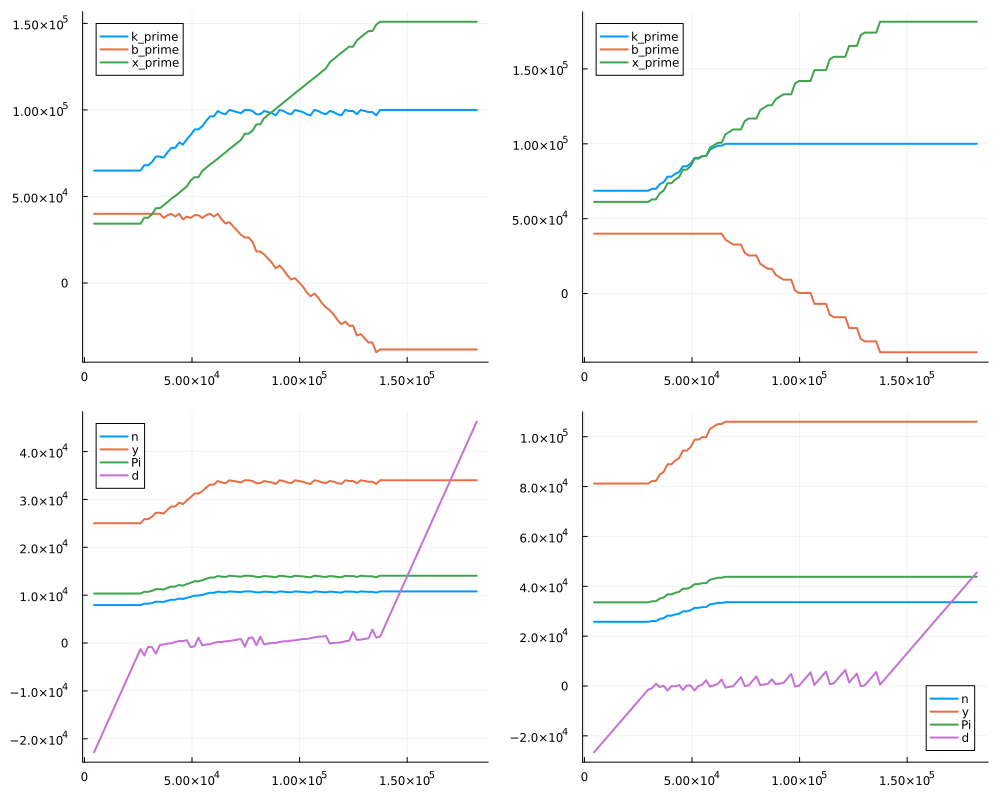
\includegraphics[width=1\textwidth]{C:/Users/szjud/OneDrive/Asztali gép/EBCs/CFL-git/Latex codes/Plots/ver2.png}
\end{figure}


\newpage
\setcounter{equation}{0}

\subsection*{Ver 3 - ABL Qs - cash on hand - AR(1) productivity}
Productivity process: AR(1) process with multiple states. Below, I plot the worst the median and the best productivity state. \vspace{3mm} \\
Labour policy: 
\begin{equation}
    n(k,\varepsilon_i) = \left( \dfrac{ \nu \varepsilon_i k^\alpha}{w} \right)^{\frac{1}{1-\nu}}
\end{equation}
Corresponding output: 
\begin{equation}
    y(k,\varepsilon_i) = \varepsilon_i k^{\alpha} \left( \dfrac{\nu \varepsilon_i k^\alpha}{w} \right)^{\frac{\nu}{1-\nu}}
\end{equation}
Corresponding profits: 
\begin{equation}
    \pi(k,\varepsilon_i) = (1-\nu) y(k,\varepsilon_i) - c
\end{equation}
Future cash on hand: 
\begin{equation}
   x' = \pi(k',\varepsilon_j')+(1-\delta)k'-b'
\end{equation}
External finance premium:
\begin{equation}
    q^{abl}(k',b')b' = \beta \left[ (1-P_\chi) b' + P_\chi \min\{b', \ \phi_k (1-\delta) k' \} \right]  
\end{equation}
Equity finance option:
\begin{equation}
    d < 0 \implies d = 1.6d
\end{equation}
Value function:
\begin{equation}
     V(x, \varepsilon_i) = \max_{k',b'}  \left( x - k' +  q(k',b',\varepsilon) b' +
            \beta (1-P_\chi) \sum_{j=1}^{N_\varepsilon} g_{ij}  V(x',\varepsilon_j') \right)
\end{equation}
Here the two innovations are that interest rates are endogenous and the productivity process is more realistic. Results makes sense, although they display this jigsaw pattern in certain regions and calibrations. \textbf{Weirdly, the model breaks down when grids are defined logarithmically.} Firms very quickly converge to their desired level of capital, even if they are cash-poor - that is because $q$ remains relatively large even for very indebted firms.

\begin{figure}[H]  % [h] indicates placing the image here
    \centering
    \caption{Ver3 - worst, median and best productivity states} \label{chart:CFLcdf}
    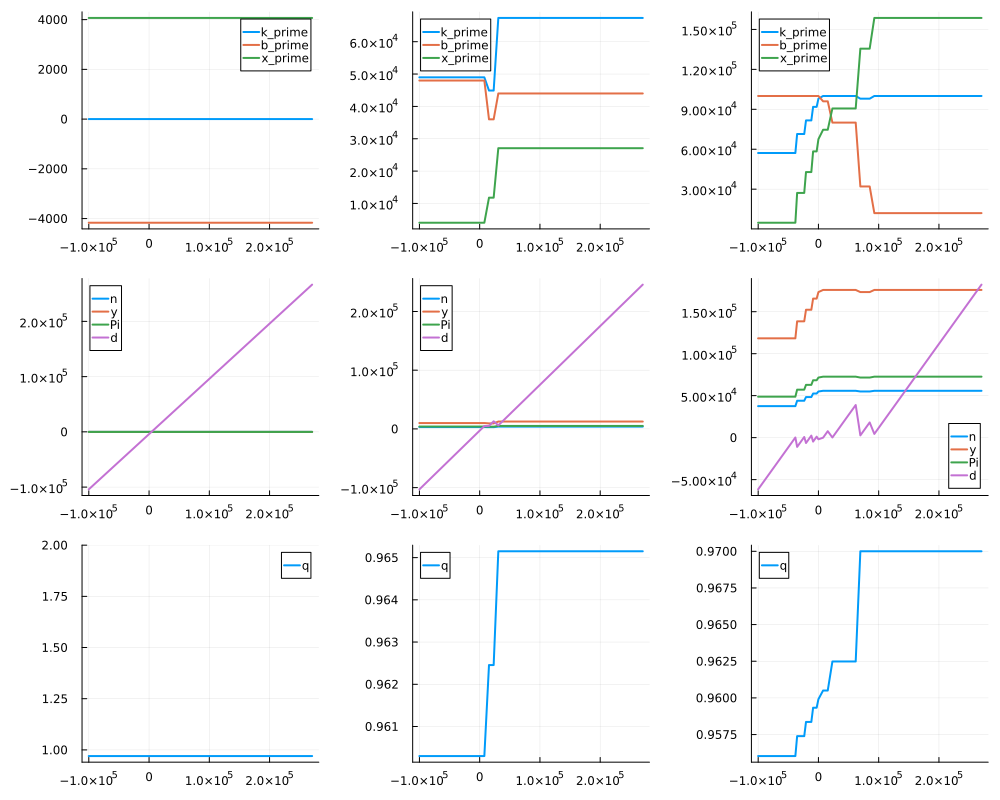
\includegraphics[width=1\textwidth]{C:/Users/szjud/OneDrive/Asztali gép/EBCs/CFL-git/Latex codes/Plots/ver3.png}
\end{figure}

\newpage
\setcounter{equation}{0}

\subsection*{Ver 4.1 - Endogenous defaults, and better x-interpolation}
\textbf{Same as in Ver 3:} AR(1) productivity process, Labour policy; Corresponding output; Corresponding profits; Future cash on hand; External finance premium. \vspace{3mm} \\
Equity finance option is not necessary anymore, but I keep it with prohibitive costs. This is needed to ensure that firms have a feasible action every state.  \vspace{3mm} \\
Default decision: the firm chooses $\sigma(x, \varepsilon)$ and the corresponding $V(x, \varepsilon)$. It chooses default if $V(x,\varepsilon) \leq 0$ and $x \leq 0$ - hence the firm can fall back to limited liability and the associated value is zero. \vspace{3mm} \\
Exit decision (not implemented in this version): the firm can decide to quit without falling back to limited liability. The associated value is the cash on hand: $x$. The firm chooses this if $V(x, \varepsilon) \leq x$ and $x \geq 0$. \vspace{3mm} \\
Value functions:
\begin{equation}
    V_0 = \max \{ V_{def}, V_{exit}, V_{cont} \}
\end{equation}
where $ V_{def} = 0$, $V_{exit} = x$ and $V_{cont}$ is
\begin{equation}
     V_{cont}(x, \varepsilon_i) = \max_{k',b'}  \left( x - k' +  q(k',b',\varepsilon) b' +
            \beta (1-P_\chi) \sum_{j=1}^{N_\varepsilon} g_{ij}  V_0(x',\varepsilon_j') \right)
\end{equation}
When a firm chooses $(k',b')$ it can expect a realization of $x$, given its current $\varepsilon$. The problem is that this may not lie on the $x$ grid. In previous versions, I chose the $x_i$ on the grid that was closest to the realization of $x$. This has led to some imprecisions. Here, I make the following adjustment: if observe the two gridpoints that surround the realization of $x$. These are defined as $x_{low}$ and $x_{high}$. \vspace{3mm} \\
Then, assume that the probability of falling on these points linearly depends on the relative distance $x_{low}$ and $x_{high}$. This yields more stable results, but computing the optimal policies becomes much slower. It is probably because the Q matrix becomes more dense when with adjustment. Also, setting up Q takes longer.

\subsection*{Ver 5 - default probabilities and endogenous interest rates}

In previous iterations of the model, the interest rate was calculated on the basis of an exogenous default probability. Now you have a default decision you can update the interest rates while taking into account the endogenous default probability. I follow the following algorithm: 
\begin{enumerate}
    \item Set $q|P_{d}(exo)$, the interest rate given the exogenous default probability. Then I calculate $V(x,\varepsilon)$ given $q|P_{d}(exo)$ - which allows me to calculate the default decision for each $(x,\varepsilon)$.
    \item Now it is possible to calculate what is the probability that the firm lands on a state $(x,e)$ associated with default. This corresponds to endogenous default probability $P_d(endo)|(x,e,k',b')$ - where $P_d(endo)$ is an $n \times m$ matrix containing the default probabilities for each state-action pair.
    \item Update interest rates taking into account the endogenous default probability $q|P_{d}(exo),P_{d}(endo)$ and recalculate the optimal $k',b$ and default policies
    \item Repeat $1-3$ until the optimal policies and interest rates do not change - that is, $ (k^{i},b^{i},\chi^{i},q^{i}) = (k^{i-1},b^{i-1},\chi^{i-1},q^{i-1}) $ for each state $(x,\varepsilon)$
\end{enumerate}
\textbf{Exit decision}: I also implement endogenous exit decision. This is analogous to the default decision, with the difference that firms may keep their cash on hand if they quit voluntarily. Moreover, you need to change the value of defaulting to some small negative value ($-1000$ in this calibration). Otherwise firms always prefer to just pay all cash on hand as dividends and stay on the market for one more period on the off chance that they receive a large, positive productivity shock. \vspace{3mm} \\
\textbf{Probability of default}: default can derive from an exogenous default shock or endogenous decision of the firm. The total probability of default can be described with:
$$             P_D = 1 - [(1 - P_{exo})(1 - P_{endo})]   $$ 
I will use this formula in the following.
\newpage
\setcounter{equation}{0}

\subsection*{Ver 6 - Heterogeneous debt contracts}
\textbf{Same as in Ver 5:} AR(1) productivity process, Labour policy; Corresponding output; Corresponding profits; Future cash on hand; Default decision, Exit decision \vspace{3mm}  \\
Value functions:
\begin{equation}
    V_0 = \max \{ V_{def}, V_{exit}, V_{cont} \}
\end{equation}
where $ V_{def} = 0$, $V_{exit} = x$ and $V_{cont}$ is
\begin{equation}
     V_{cont}(x, \varepsilon_i) = \max_{k',b'}  \left( x - k' +  q(k',b',\varepsilon) b' +
            \beta (1-P_\chi) \sum_{j=1}^{N_\varepsilon} g_{ij}  V_0(x',\varepsilon_j') \right)
\end{equation}
External finance premium: 
\begin{equation} \label{eq:opt_tau}
    \begin{split}
        & q = \frac{\beta}{b'} \Big{[} (1-P_D)b' \ +  P_D \Big(\min \big\{ b', \ \  \gamma(k',b',\varepsilon) \left( (1-\tau') \phi_A (1-\delta) k' +\tau' \kappa \phi_A  (1-\delta) k' \right)  \\
        & \quad  +  \ (1-\gamma(k',b',\varepsilon))\left((1-\tau') \phi_A (1-\delta) k' +\tau' \left( \phi_C \E_{\varepsilon'|\varepsilon}V_2 (x', \varepsilon') - \zeta \right) \right) \big\} \Big) \Big{]} 
    \end{split}
\end{equation}
The firm has access to CF-based and asset-based debt contracts simultaneously. It chooses the optimal reliance on CF-backed debt, $\tau$ to maximize $q$. Therefore, the $\argmax$ of equation 3 describes optimal CFL reliance. The solution strategy is the same as in version 5, but now it is much more complex, hence it is also more prone to error.
\begin{enumerate}
    \item Set $q^0$, the starting interest rate at $\beta$ and calculate the value of the firm, $V(x,\varepsilon)$ and $k', b'$ and exit policies given  $q^0$. 
    \item Calculate the following: the probability of default $P_D$, the probability of liquidation under default $\gamma$, the liquidation value; $\phi_A (1-\delta) k'$ and the reorganization value; $V_2 (x', \varepsilon') - \zeta$ given $q^0$, for each state-action pair - meaning that all these are $n \times m$ matrices.
    \item Update interest rate, $q^1$ associated with the state-action pair, taking into account the default and liquidation probability and lenders in-default payoffs. To do this, you also need find $\tau^1$ what maximizes $q^1$ for each state-action pair. This requires an additional loop, that calculates $q^1$ given tau, and then chooses the best $\tau$.
    \item Repeat $1-3$ until the optimal policies and interest rates do not change - that is, $ (k^{i},b^{i},\chi^{i},q^{i}) = (k^{i-1},b^{i-1},\chi^{i-1},q^{i-1}) $, or at least within some tolerance value for each state $(x,\varepsilon)$.
\end{enumerate}
\textbf{Issues of non-convergence}: sometimes this model version does not converge. There might be two reasons for this. First, it might be that the next $x$ with a particular debt decision falls closer to the non-default $x$ on the grid than the one associated with default. Then the lender offers the borrower a low interest rate even though the debt policy is not sustainable. In this case, the iteration is cut short. A quick solution is to increase the x-grid. A better one would be to do the same Xlow-Xhigh setup as in the Q matrix - \textbf{already implemented and it solves most convergence problems}. Second, the model practically converges, but there is oscillation between two neighboring debt levels and corresponding q-s. This can be solved with increasing the $b$ grid. Alternatively, you can just write a code that stops after this oscillation starts. Not very elegant but it is ok.



\newpage

\subsection*{Finding the stationary firm distribution}
Solution approach:
\begin{itemize} \setlength\itemsep{0em}
    \item Set up the VFI to find optimal policies given state variables and the wage, $w$ (some models solve for the price of the final good $p$, I use price as the numeraire so I can solve for the wage)
    \item Equilibrium wage is such that the value of entering is equal to the cost of entering: $V^e = k$ - this works only with entry decision 2. (see below)
    \item The stationary distribution is defined as follows in matrix form 
       $$ \mu = F(I-\text{diag}(X)) \mu + mf^0 = M\mu + mf^0 = m(I-M)^{-1}f^0 $$
       where $\mu$ is the distribution of firms, F is the transpose of the transition matrix given productivity shocks and policies; X denotes the exit policy; $f^0$ is the vector of entrants and $m$ scales the distribution of firms
    \item Defines the transition matrix of incumbents given production and exit policies and the productivity transition matrix $\rightarrow$ M
    \item Takes the vector of entrants $\rightarrow f^0$; in my model entrants may exit immediately, so $f_0$ should also be premultiplied with $I-\text{diag}(X)$
    \item The unscaled stationary distribution of firms ($\mu^{0}$) can be expressed as: 
        $$\mu^{0}= (I-M)^{-1}f^0$$
    \item Finds $m$ from labour market equilibrium given wage; 
        $N(w) = m \sum_\varepsilon \sum_x \mu^{0}_{x, \varepsilon} n_{x, \varepsilon} $
    \item Scales the stationary distribution $\mu = m\mu^0$ $\rightarrow$ $m$ is the measure of entrants but it scales the entire stationary distribution
\end{itemize}
 \textbf{On entry decision}: this must be figured out in order to have a stationary distribution of firms. In the Hopenhayn model the entry decision is made ex-ante, before learning about your productivity. Therefore, the value of entering is the same $V^e$ for each potential entrant. Under the free entry condition, $V^e = k$. I set up the model such that potential entrants first learn about their state and then decide to enter or not. This setup is designed to study composition of entrants under aggregate shock - as in Khan and Thomas. \vspace{3mm} \\
I see 3 ways:
\begin{enumerate} \setlength\itemsep{0em}
    \item Entrants decide in full knowledge of their ($x, \varepsilon$) - KT16, Kaas22
    \item Entrants decide ex-ante, knowing only $V^e$ - Hopenhayn, CandD
    \item Exogenous flow of entrants - Leo's recommendation, KT13, Öztürk (2023)
\end{enumerate}
Number 1 and 2 can be made almost equivalent setting the timing such that entrants do not produce in the current period. In this case, potential entrants uniformly face $V^e$. Then, they receive ($x, \varepsilon$) and can decide to exit, default or continue just as the rest of the incumbents. Hence, nonviable young firms exit after one period instead of not entering at the first place. The only difference to approach n1 is that it adds to the default and exit rates, but you can use the solution approach from above! \vspace{3mm} \\
Alternatively, you could have entry in the beginning of the period after which startups produce and decide to exit and or default. This is almost the same except that entrants take part in production. \vspace{3mm} \\
\textbf{Entrants' problem}: \\
There is a mass ($m$) of potential entrants that may enter after production has taken place. Entry decision is informed by the free entry condition, $\beta E[V^e(x,e)] - c_e = 0$ where $x_e$ the starting cash on hand and the $c_e$ is the setup cost. This decision takes effect at the end of the period, so firms quit without ever taking part in production. In this setting, entrants' problem is the same as incumbents', but their value is discounted by $\beta$ due to the timing. \vspace{3mm} \\
Define the joint starting distribution of $\Gamma(x,\varepsilon)$. Since $(x,\varepsilon)$ are independent in the beginning, you can just define the two distributions separately. The common practice is to set entrant productivity distribution equal to the stationary distribution implied by the Markov Chain. Having an entry cost also justifies setting a $x_e$ distribution with negative values. In this case, the firm co-finances entry with the household. If the firm decides to exit without taking part in production the household gets $x_e - c_e$, meaning that $c_e$ is treated as a sunk cost. \vspace{3mm} \\
An interesting approach is to set the entry cost such that the equilibrium wage is equal to 1. Then you would not have to mention the large entry cost in the calibration - although this is not necessarily a problem. For now, I am choosing x=0 for all entrants because it is clearer. However, you might want to consider the x-distribution approach later, that might yield larger effects on the intensive margin. \vspace{3mm} \\
\textbf{In the current model}, entrants enter at the beginning with $x = 0$ (to keep things simple), they do not take part in production but may pay dividends and exit or default. These assumptions ensure that they face the same optimization as incumbents, so I do not have to solve a separate VFI for entrants. Their entry cost $c_e$ and starting cash on hand $x_e$ is financed by the household. If they exit or default immediately $x_e$ is rebated to the HH and $c_e$ is lost. This implies a stationary distribution of:
$$ \mu = F(I-\text{diag}(X)) \mu + m(I-\text{diag}(X))f^0 $$

\subsection*{Misallocation}

The best reference for studying misallocation in this model framework is Kochen (2022), since his approach is very similar to mine. He also measures productivity as Y/L and he also finds that this is proportional to the wage. This means that everything that changes the wage affects aggregate productivity in the end. Moreover, he gives an easy solution to find the perfect credit equilibrium by simply making equity finance free. In my model, this amounts to getting rid of the $d \geq 0$ constraint.  \vspace{3mm} \\ 
Decomposes the reduction in productivity to reduction in TFP and reduction in capital deepening: 
$$ Y/L = \text{TFP}^{1/1-\alpha}(K/L)^{\alpha/1-\alpha} $$
Taking logs, it is possible to decompose this into the effects of capital deepening and TFP. Then, he further decomposes reduction in TFP into misallocation of capital (reduction of due to dispersion of capital-output ratios) and distortions in the mass of active firms. He finds that the latter effect dominates. I could do this decomposition but it probably does not add that much to the results overall. However, it means that I should focus on the reduction of productivity rather than the misallocation of capital.

\subsection*{Partial Equilibrium or General Equilibrium}
In partial equilibrium, there is no household and no prices (goods prices, wages and interest rates) are set externally. This is not what I am doing in the model. Labour market clearing is achieved by simply adjusting the mass of firms such that $N^s = N^d$ holds, where $N^s$ is the inelastic labour supply of the household. This already assumes there is a supply of labour - even if it is inelastic. Hence in this part, the model is GE. \vspace{3mm} \\
Moreover, wages adjust such that the entry value of the firm matches the fixed cost of entering (free entry condition). If wages are not allowed to adjust, then the cost of entering must adjust in order to keep up the free entry condition. This might still be valid, since total labour is just some number, which may give you some freedom in always normalizing wage to zero. On the other hand, my results depend on the wage changing so I might not want to consider this. \vspace{3mm} \\
For a GE model, you need 3 markets that need to clear: labour, bond and goods. Labour market clearing is easy to achieve by setting the mass of firms. The other two are not as straightforward. If you follow Corbae and D'Erasmo you can say that goods market clearing is ensured by Walras' law (HH budget constraint holds with equality) such that consumption is whatever left from output that is not invested or lost in production (adjustment costs, fixed costs of operating, capital sales from exiting firms, bankruptcy costs etc). This is in fact not so far from my assumption that consumption passively adjusts to $C = Y - I$, but it also takes all the leftover costs that are present in the economy. The same logic is followed by Di'Nola, Kaas and Wang so taking this approach should be fine.  \vspace{3mm} \\ 
As for bonds market clearing, you need to discuss two things: first, it can be derived from households' optimization risk free interest rate of bonds must be equal to households intertemporal marginal rate of substitution. That is $q_0 = \beta$. Moreover, market clearing on the bonds market requires that firms' discount factor corresponds to households the same marginal rate of substitution. It seems that once you have these, it is enough to assume that $B^s$ adjust passively. The way to think about it is that in this case you already have $B^d$ and prices pinned down. Moreover, your assumptions make sure that the bond market clears, so $B^d = B^s$ must hold. \vspace{3mm} \\
Note that when setting the household and firms discount equal to each other, the covid paper argues that this firms values represent marginal contributions to the households' utility; therefore dividend payments accrued in the next period are priced by the financial discount factor of the household. This seems more intuitive, so maybe it is enough to mention this when using $\beta$ in firms' optimization.

\subsection*{The productivity process (Tauchen's method)}
Productivity follows the AR(1) process:
$$ \ln(\varepsilon_{t+1}) = (1-\rho) \ln(\varepsilon_0) + \rho \ln(\varepsilon_t) + \sigma \zeta_\varepsilon $$
\begin{itemize}\setlength\itemsep{0em} \small
    \item $\rho$ is the persistence of the shock
    \item ln($\varepsilon_0$) is 'average productivity'm calibrated to $1$ in Kaas et al.
    \item $\sigma$ is the standard deviation of shocks
\end{itemize} \normalsize
I discretize the log-process via Tauchen's method, then take the exponents of the productivity values. This process does have some mean reversion in it, due to the first term on the RHS - however not every paper have this term, KT13 for instance does not. Moreover, I found two calibration approach: in Kaas, Öztürk and Kochen it is high persistence with $\rho$ close to one and small innovations whereas with KT13 and CandD, $\rho$ is around $2/3$ and innovations are large. In these papers there is no reversion to the mean in the AR process. Overall, I am not a hundred percent sure how to best set it. 

\subsection*{Calibration}
\begin{itemize}\setlength\itemsep{0em} \small
    \item First find the data moments that you want to match - must be reproducible in the data and in the model
    \item Then find the parameters you are that affect these moments the most without affecting other moments too much - you must have at least as many moments to match as the number of parameters (otherwise there are infinite solutions)
    \item Then, set a function that transforms the deviation of model values from their targets into a single value - sum of percentage deviations seem perfect
    \item Take the entire model as a function that takes the parameter values and produces the target values into the loss value defined by the function above. 
    \item Finally, send it into a solver. `Optim' package is good, you can use Nelder-Mead algorithm that requires no differentiation or LBFGS which differentiates which makes it faster but less robust.
    \item Try to keep the model solution time at a few minutes to make the calibration run in time. 
\end{itemize} \normalsize


\newpage

\subsection*{Interpretation of model results}
\textbf{Entry on the extensive margin.} I study if CF-based borrowing affects the extensive entry margin for firms. I find that there are no significant differences between the ABL and the CFL case - this somewhat contradicts preliminary runs. However, this is not such a big shortcoming, with the current calibration productive firms still enter with around -20000 of cash on hand. There is no realistic way to justify this sort of cash on hand upon entry. \vspace{3mm} \\
\textbf{Comparing ABL and CFL case.} I extend the calibrated model version where firms only have access to ABL debt (ABL-case), to the model where there may choose either (CFL-case). Sanity check: the CFL case where the cost of CFL is prohibitive is equivalent to the ABL case. The differences are the following: 
\begin{itemize}\setlength\itemsep{0em} \small
    \item When firms do not have access to CFL debt, they often hold more capital. This can occasionally be seen on the long-run. Firms hold more capital after they have reached their optimal size when there is no CFL lending available. This is even more pronounced when firms enter the market with negative cash on hand. In this case, they can pay their previous debts only if they buy a lot of next periods' capital, which gives them access to a lot of debt.
    \item The main difference between ABL and CFL cases, is that in the latter case the most productive firms have a better access to external finance, which means that they rarely borrow for a $q$ much different from $\beta$. This allows them to pay higher dividends and realize higher values. However, this does not always realize in higher capital or debt - this may be partly explained by the incentive to over-borrow in the ABL case, but its also possible that the grid is not fine enough. Later, in firms' life-span these differences evaporate as firms become unconstrained.
    \item Large recovery rates for banks also implies that firms can run a bigger chance of default without increasing the external finance premium too much.
    \item The largest effect could be through the change of values, with changes the entry decision and affects wages. These effects are probably not huge but still considerable. If you want to increase the effect of CFL lending on the stationary equilibrium, consider calibrations that change the value of entrants.
\end{itemize} \normalsize
\textbf{Dynamic Simulations} 
I take an entrant with a certain productivity and simulate their path given Fmat - the transition matrix of incumbent firms. Then, I repeat this simulation a large number of times and take averages - these show the average path of a firm that enters at a given productivity. The path of x, k, b, y, d and v  are intuitive, the reason for the decline at large productivities is a results of the mean-reversion of the AR process. \vspace{3mm} \\
The issue is with comparisons: I compare firm dynamics when there is access to CF-based borrowing and when there is none. I find that firms that are not the highest productivity state (but still have access of CF-based borrowing) are smaller (smaller production, capital and value). The reason behind could be that I assume a fixed wage in the process, which implies that the entry cost is changing. Meaning, that I do not run the model on the same parameter values. This shows on the steady state values.  When there is access to CFL, firms are on average smaller and produce less but hold more debt. \textit{Maybe comparing them when entry cost is fixed and wages are different would be a better idea - but even then you could not control for changes in average firms sizes.} \vspace{3mm} \\
\textbf{Results around liquidation probability} \\ 
\begin{itemize}\setlength\itemsep{0em} \small
    \item Xcross: Show that CFL reliance decreases as the liquidation probability increases - this could be even made into an untargeted moment. \checkmark
    \item Aggregate productivity for different calibrations: No credit access, Only ABL, Baseline, Low reorganization costs, Perfect credit.  \checkmark
    \item What is the external finance cost if there in the ABL vs Baseline case and maybe even a Low reorganization cost case. This plot shows the differences between having access to CF-based debt vs not. Could be done either for average of optimal firm policies (\checkmark) or in hypothetical scenarios.
    \item How does optimal debt financing strategy changes as liquidation risk increases. Make a plot where size is on the x-axis, productivity on the y-axis and coloring shows the $\tau$ - then do this for high and low liquidation probability. 
    \item How does external finance cost changes as liquidation risk increases. Here, you need to fix $(x,\varepsilon,b)$ and just make liquidation probability change. You can also take a high and low productivity firm as an example. 
    \item \textbf{Loosely related}: Histogram of CFL reliances, how external finance changes with other firm characteristics, optimal policy changes with firm characteristics. Dynamic simulations: optimal average policies over the lifecycle. 
 \end{itemize} \normalsize

\newpage

\section*{General Notes}
\textbf{Ex-ante default probability} \\ 
In the current model, default probabilities are endogenously defined by the expectation of the liquidation decision. However it seems that endogenous $\gamma$-s complicate the model a lot. First, a model where these cannot be set, must be adjusted through $\zeta$ and $\phi_c$, which is more cumbersome. Second, sometimes it yields weird results. For instance, in a case where reorganization costs are prohibitive, the lender can predict with certainty that the firm will be liquidated, which may even yield more relaxed credit conditions - \textit{probably this effect is not very strong though}. \vspace{3mm} \\
Fixed liquidation probabilities would probably yield a more stable model. How to implement these, probably the best approach is to look at the production of firms and fit a decreasing curve through it that is informed by IDB data. How to do it in practice is less obvious. \vspace{3mm} \\
\textbf{Measure of size problem} \\
The cash on hand approach does not have a good measure of current size. The current cash on hand might be misleading since large debt might cancel out large capital stocks. You could do next periods' expected cash on hand, or next period's capital stock. Or simply just take current capital into account. \vspace{3mm} \\
\textbf{On interest rates} \\
You can rarely see default probabilities over 4\%. This does not mean that financial frictions are not significant. This is because the probability of default jumps at some point at a certain debt policy. This implies very high interest rates, which is not a good deal for the firm. Therefore in most cases, firms stop short of high levels of debt that would increase their default probabilities too much. \vspace{3mm} \\
\textbf{On debt debt policy of firms} \\
Iff defaults are exogenous and associated with zero value, firms discount future by $\beta(1-P_\chi)$, whereas the fully secured interest rate is $\beta$. Therefore, when the firms manages to be fully secured, it prefers to hold a lot of debt and pay higher dividends, because if it defaults next period it might loose the accumulated cash on hand. This implies that even large, cash rich companies hold a lot of debt. Not a bad result, but probably not for the right reasons. \vspace{3mm} \\
\textbf{Firm growth} \\
Firms grow very quickly to their efficient sizes. A firm with no cash on hand has easy access to a lot of debt, and can grow out of cash-poorness very quickly. This is a problem if I want to focus low wealth but productive firms. \textit{Yes, this is an issue here, but it is an issue in pretty much all the models like this.} \vspace{3mm} \\
\textbf{Exogenous Default - with option to exit} \\
Having this in the model means that firms have no incentive to accumulate cash on hand. This implies that firm growth basically typically happens in 3-4 period. After that point the firm has no incentive to accumulate more cash on hand and is effectively unconstrained. Therefore, it might be interesting to consider cases where, there is no exogenous default (set Pdef-exo = 0 or take it out of the discount). If you do this firms accumulate cash on hand over time. They use this to finance capital investments, so they do not need to hold debt (in this case negative debt may make more sense). However, firm reaction is not linear, at some point firms decide to limit production in order to accumulate cash flow faster. This leads to a wobbly dynamic behavior which is not really nice. This should be better explored but I am not sure how to do it practically. \vspace{3mm} \\
\textbf{Conceptualizing negative cash on hand for entrants} \\ 
How would a firm enter with negative cash on hand? You can add entry costs (usually they are needed anyways). You can assume that firms need initial financing to pay entry costs. This means that cash on hand is bounded from below at minus the entry cost. This is needed if you want to have cash poor but productive firms in the model. \vspace{3mm} \\
\textbf{The linearity of q in CFL reliance} \\
The expected in-default payoff of the lender after the asset-based debt is: 
$$  (1-\tau') \phi_A (1-\delta) k'  $$
for CF-based debt: 
$$    \tau'\left[\gamma(k',b',\varepsilon)(\kappa \phi_A  (1-\delta) k') +  (1-\gamma(k',b',\varepsilon))\left( \phi_C \E_{\varepsilon'|\varepsilon}V_2 (x', \varepsilon') - \zeta \right) \right] $$
The borrower chooses $\tau$ to maximize the sum of these two values. Since both of them depend on $\tau$ linearly, the optimal decision on $\tau$ is 0 if the first sum is larger and 1 of the second sum is larger. Hence, this setup still cannot reproduce CFL reliance in the range of $(0,1)$. \vspace{3mm} \\
The solution would be to add a $\gamma$ that increases in $\tau$. That is, higher reliance on CF based lending increases the chance of liquidation. This is realistic if the borrower can keep whatever is left after the default process and it gets to decide on liquidation. An example would be that a firms with a lot of unsecured debt chooses liquidation since lenders cannot enforce liquidation payments. this could deliver results, but it is not very realistic. \vspace{3mm} \\
\textbf{Optimizing the code}: \\
The most time is taken by the loop where you update the values, default probability etc - this is only getting worse if gamma has to be calculated in a separate loop. One solution to this would be setting the number of threads to maximum. I found that on a single loop this cuts computation time to around 1/3rd. However, once I integrate it into the big function this gain is lost. This is because threads does not seem to work well in nested loops. ThreadsX supposed to do better in this, but it does not lead to any development either.  The other option to juice up the performance a bit is to define the data type of the parameter values. This seems to add some to the performance but its not a huge change.
\vspace{3mm}\\
\textbf{Taking logarithmic grids} \\
Results with logarithmic grids are not perfect, but they generally make sense. The problem is that some low cash on hand firms prefer to just produce a lot in the current period without accumulating assets - their production is financed by external finance almost entirely and their next period cash on hand is stuck at a low value.  This is especially true for high productivity firms. \vspace{3mm} \\
This is not a bug (see the steadily increasing value in $x$) and it is not necessarily a problem, but it is a bit weird that firms of the same productivity do not converge to the same cash on hand - should check it under CFL borrowing. I should also add that this in every calibration, under some certain values very few firms actually do this. Making the discount parameter closer to one would probably solve this problem.   \vspace{3mm} \\
\textbf{Allowing for financial savings} \\
Allowing $b$ to be negative means that a lot of firms with low productivity but high cash on hand do not exit immediately, but dismantles capital stock gradually. This would yield a gradual decline of financial wealth. Overall, results are nicer and converge faster, but of coarse the grid becomes less granular. With log grids and negative financial savings the model does not converge.  \vspace{3mm} \\
\textbf{Firm dynamics - Fmat fix} \\ 
Earlier model version Fmat does not take into account exits in firm dynamics. This does not affect optimal firms choices (those are informed by Q and R) but it affects stationary distribution. Big masses of firms pile up in weird steady states that are associated with high liquidation probability. In later versions (up from ver7.2) this is fixed. Transition values in Fmat are scaled down with the endogeneous default probability, and a separate column for default-state is added. Overall the differences after the update are not large, but still visible. \vspace{3mm} \\
\textbf{The determinants of firm size} \\
 The Lukas type span of control parameter, and the price of the final good are the best to limit firm size. If you want more firms to participate (and firms participate from a lower cash on hand level) decrease the participation cost of entering. \vspace{3mm} \\
\textbf{Fixed costs} \\
Cost of reorganization is pretty much a given in the model. However, it is not clear whether it should be imposed on the lender or on the borrower. If the liquidation decision is made optimally by a third party, it should not matter who pays for it. But, you might be able to get a more direct effect on the  availability of CF-based debt if the lender is directly affected by this fixed cost and not just through the liquidation probability. Fixed costs of liquidation are used by Corbae and D'Erasmo. It is not necessary for the model mechanism but it may help to reproduce some moments in the data. These are the U-shape, meaning that small firms often borrow against cash flows, and the average CF-reliance. \vspace{3mm} \\
\textbf{Default shocks} \\
Currently, default shocks are modelled as a negative shock to productivity that is always associated with either default or exiting. This means that even the most productive and largest firms default with some probability. The problem with the current model setup is that it considers the unconditional probability of reorganization, whereas it should consider the probability \textit{conditional} on default. However, fixing this introduces further problems as no (or very few) firm would choose reorganization at the end of a voluntary default: since the value or reorganizing is always lower than the value of continuing. What could save this if reorganizations  would happen under involuntary default. However, it is also very unlikely that a firm would receive a negative shock such that it could not repay its debts but still productive enough that it wanted to continue. \vspace{3mm} \\ 
To make this occurrence more frequent, make the negative productivity shock temporary such that there is a `modifier' to productivity which is 0 with some probability - P-exo. This would allow productive firms to be hit by a shock such that they want to reorganize and still allow for endogenous defaults. To implement this, you have to add a separate markov chain that has values: $[0,1]$ and a transition matrix that describes the random shock occurring with `Pdefexo' probability.  Note that you have to update the grid sizes accordingly. This introduces a problem, as the size of the `Q' matrix doubles, so I run into memory issues much faster - \textit{This might not be true, maybe there is a way to rewrite the Q matrix instead of the productivity process.} Luckily, the runtime does not change much probably because the zero productivity values are easy to calculate.  \vspace{3mm} \\
Alternatively, I could choose exogenous default shocks where firms are sometimes (exogenously) forced to choose between liquidation and reorganization. This would simplify the model a lot because the conditional and unconditional probability of default would be approximately equal. Then reorganizations and liquidations could be imposed outside the main loop, on the FMat matrix. \vspace{3mm} \\
It seems now that the solution is some combination of endogenous default decisions and exogenous default shocks - although the description of this would be quite weird to justify in the model. You do not have to worry about the timing of these shocks. In the stationary equilibrium the share of firms that chose a certain $(k,b)$ policy is the same that did so in the previous period. Therefore, in the code, it is enough to just look at current incumbents optimal policies to know the previous incumbents' decisions, which allows you to calculate liquidations and reorganizations. This implies that exo shocks can materialize at the same time as endo shocks.  \vspace{3mm} \\
The shortcoming is that now the model would have involuntary and voluntary as well as exogenous default shocks. This would not look so good in the paper, although it is not necessary to make the distinction between voluntary and involuntary defaults. You could also just try to kill endogenous default and see how it affects policies - but the problem with this is that in this case the model does not have a good answer what happens to firms that cannot find a debt contract that would allow them to repay their previous debt and pay non-negative dividends at the same time.
This could be solved by adding a costly equity finance option. \textbf{This is something to try later.} \vspace{3mm} \\
\textbf{Liquidation probability is a function of CFL reliance} \\
This iteration requires an extra loop nested in the variable updating loop - since now $\gamma$ and $\tau$ are jointly determined, you need an extra loop to solve them both. This increases computation time, but not by a lot. The benefit of this is that now $\tau$ is not a corner solution, so the model can reproduce $\tau \in (0,1)$ too. The gains from liquidation and reorganization can still be redistributed to the household or given to the firm. \vspace{3mm} \\
I find that: the distribution of CFL reliances is reproduced quite well, such that there is a bunching at values $\tau = 0$ and $\tau = 1$ and some observations in the middle. One caveat is that $\tau = 1$ is mainly driven by huge firms that have a zero probability of default. For these firms, I assume that they chose CF-share of 1 if their reorganization value is larger than their liquidation value. The share of CF-debt in the economy would be relatively easy to match.   \vspace{3mm} \\
The big problem is that the model does not react monotonously to changes in $\zeta_R$. For instance if you set $\zeta_R = 8000$ the CF-share is 0.73, but if set $\zeta_R = 6000$ the CF-share drops to 0.68, if you decrease $\zeta_R$ further CF-share sometimes increases. The one thing suggesting consistency, is that the gainst from CF-based borrowing always increase as I decrease $\zeta_R$ Due to the feedback of $\gamma$ and $\tau$ the whole mechanism is a bit confusing. \vspace{3mm} \\
\textbf{How to rewrite code when Vdef is not equal to zero?} \\
It now seems that it is not possible to calculate these in the QuantEcon setup without considering $(k,b,\varepsilon)$ as state variables. The problem is that to decide if a firm would choose liquidation or reorganization, you would have to know $k,b$ in default. However this is not possible to calculate with only $x,\varepsilon$ as state variables. Added complication is that for reorganization you also need to know the value of the firm, but the value in reorganization affects the value in the first place. This can be embedded in the main loop but the convergence properties are questionable. \vspace{3mm} \\ 
Furthermore, if you make the either liquidation or reorganization value dependent on $\tau$, it is no longer true that the $\tau$ that maximizes $q$ is the optimal. In this case, you need to consider an additional decision variable, as in ver8.3. This might add too much computation cost. Alternatively, you can consider a setup where the value of liquidation for the firm is always zero and the value of reorganization is fraction of the continuation value minus the fixed cost. This can be made consistent with the lenders payoffs by assuming that whatever is not taken by the lender and not gained by the firm is simply a welfare loss. This way, default value does not depend on $\tau$, so it is enough to search for optimal CF-reliance in a simple loop.  \vspace{3mm} \\
\textbf{Issue of reorganizations} \\
\textit{Note that you do not have this issue if reorganizations happen only exogenously! Moreover, since it only affects the stationary distribution of firms and there are very few reorganizing firms to begin with, this is the kind of issue that would change the results very little once fixed.} \vspace{3mm} \\ The model assumes that with default, the firm decision on future values of $k$ and $b$ does not matter. This eases the computational burden, since you do not have to multiply the size of the decision matrix - the [k,b] grid - only add two lines to the bottom. One for default and one for exit. However, this is not true when firms may choose reorganization in default. In this case, they continue to the next period and they must make decisions on (k,b). \vspace{3mm} \\
The honest thing would be to add exit, liquidation and reorganization as separate decision variables, and then allow reorganizing firms to choose any value of (k,b). But this would double the size of the (k,b) grid for reorganization \{0,1\}. This would probably be too much computationally. One way around this would be to assume that reorganizing firms do not exit but they must choose $k',b' = 0$. This would imply a next period cash on hand close to zero and a productivity that is defined by the AR(1) process. This could work but it is a bit patchy and it would complicate the Vdef issue. \vspace{3mm} \\ 
\textbf{Big problems right now}
\begin{itemize}
    \item How would it be possible to decide between liquidation or reorganization without adding an extra state variables
    \item How to match the share of reorganizations without making the default decision and productivity shocks too complicated
    \item How to solve the VFI in the QuantEcon package if the value of default is not zero universally.
\end{itemize}
 
\newpage

\section*{Comments}
\subsection*{Leo's comments}
\textbf{Minor Comments}:
\begin{itemize}\setlength\itemsep{0em} \small
    \item Make punctuation at the end of equations consistent
    \item Do not mention limitations in advance of the empirical or structural model - make them into a footnote, or leave it to the discussion of the follow-up work
    \item Confused about who takes what (no HH in the model):  leave the household out of the explanation here, better to give the leftover to the firm. This would actually simplify the explanation of the model, since the firm is the logical place where the leftover value should end up.
    \item Confused about the liquidation and reorganization. The firm is either fully liquidated or fully reorganized no in-betweens. Maybe a flow chart would help elucidating the process. 
    \item In case of continuation, the household retains an operational firm which is associated with a continuation value of $V_{cont}(a',\varepsilon')$. This it does not actively `gets' anything, just retains some future continuation values. I think this would be much clearer if I rewrote with firms. 
\end{itemize} \normalsize
\textbf{Minor Comments 2}:
\begin{itemize}\setlength\itemsep{0em} \small
    \item Write out the condition for forces default
    \item Figure out the expectations terms in the lender's zero profit condition
    \item Try to shorten lenders' expected payoffs section
    \item The values in the table are misleading - they actually should be expressed per unit of debt
\end{itemize} \normalsize
\textbf{Options to consider}:
\begin{itemize}\setlength\itemsep{0em} \small
    \item When a firm is reorganized the asset-based lender still liquidates assets and the CF-based lenders receives only the continuation value of the firm with reduced assets: this has some merits since liens on all assets are set up like this, on the other hand it invalidates a lot of what I argue before with the best interest of creditor test
    \item To make the model internally consistent, use an exogenous default shock and two options under default: liquidation and reorganization; and two options under no default: exit or continuation. It would be possible to avoid an extra state variable in the main optimization, since $b$ would only matter for the firm when it was in default. Therefore maximizing $V_{cont}$ would be unaffected by current $b$ but firms could take into account that $b'$ affects the value in default - \textit{this is what Leo refers to as well.} \vspace{3mm} \\
    Maybe, this could be done with just negative shocks - in this case the borrower would only choose reorganization if it could not repay its debt!
    \item Consider a model where the borrower has to pay some share of the debt to the lender in case of reorganization
    \item Maybe it would be better to emphasize the two most important simplification assumptions: there is only a single lender and only two types of debt contracts. It would be easy to argue that any deviation from this would increase the complexity of the model a lot. 
    \item Probably it would be best to start with the assumptions of lenders in-default payoffs. 
\end{itemize} \normalsize

\subsection*{Marek's comments}
\begin{itemize}\setlength\itemsep{0em} \small
    \item For faster convergence, try relaxing the convergence criteria in the while loop. Do not deed to do it until numerical precision - \textit{not sure it would help too much but worth a try}
    \item Check Julia Profilers 
    \item Do typesetting for every variable not just the parameters
    \item You need at least as many moments as parameters, otherwise you parameters are not well defined - \textit{this should be especially important when it comes to solving the calibration with a solver, see below}
    \item When you do calibration, just put the entire model as a function, with parameter values as inputs. Then set a distance from target as an output of this function. Finally, choose a solver that minimizes this distance. 
    \item When setting moments to target, look at BDS and Compustat values. Then choose a linear combination of these targets depending on how close the firm distribution in your model is to BDS versus Compustat. 
    \item You could match to average size - \textit{although measuring anything in efficiency units of productivity you can scale up or down the entire as much as you want}
    \item Consider not reporting wages at all - same for exit rates. These would just invite some unwelcome questions.
    \item The model is actually dynamic, it just lack aggregate shocks 
    \item Firm age is actually important in the model! - even though you do not have this in explicitly in the model, it matters because as there is really no other way for a firm to be young and productive at the same time - \textit{maybe add extreme positive shock to reduce this issue}
    \item Think about the story you are telling, not just the results - what happens and why!
    \item Is this a GE or a PE? In PE prices should be the same so it is not consistent with talking about wages in this case. Wage changes in the model is possible because actually there is an equilibrium for this market the only assumption is that labour supply is fixed. On the other hand, consumption and savings just react passively such that prices are 1 and savings react passively such that the risk free rate is 0.03\%. However, this is not good. If you really want a PE you cannot just have them adjust passively.  
    \begin{itemize}\setlength\itemsep{0em} 
        \item How to set B - value: Khan and Thomas 
        \item How to set consumption
        \item How to set PE? - Kochen; C\&D; Credit Growth
    \end{itemize}
    \item Low cost of reorganization may also be good because it allows small firms to stay on the market when they experience financial distress. How is this calculated in the model? Is it even taken into account. This should be considered but it could be turned into a feature. 
\end{itemize} \normalsize

\subsection*{Seula Kim's comments:} 
\begin{itemize} \setlength\itemsep{0em} \small
    \item Try interpolation between grid points 
    \item Seeing misallocation on the extensive margin would be interesting
    \item How firms choose debt financing strategy? Make a chart with optimal CFL reliance depending on liquidation risk
    \item Learning frictions in the model would be interesting: lenders would have to learn borrowers' productivity - this would allow them to lend against future cash flows (in general, she seems to be interested in information frictions, she has something similar with firms and workers). 
\end{itemize} \normalsize 

\subsection*{Nicolo's comments:} 
\begin{itemize} \setlength\itemsep{0em} \small
    \item \textbf{Intro}: Introduction is too long - move the literature slide to the intro of the intro, try to rephrase the first slides in a flow chart that explains what you do vs. the literature
    \item \textbf{Intro}: Drop the formulas from the intro, its too early for those (use `only' in Latex)
    \item \textbf{Intro}: Then research question - one at a time: first discuss micro level optimal policies, then on the next slide move on to aggregate implications 
    \item \textbf{Empirical part}: Do not highlight in red because that usually implies mistakes - use some light blue
    \item \textbf{Empirical part}: Probably best to talk little of the empirical results since it invites a lot of questions and you probably want to focus on the model part.  Just a quick summary of the main results, and then justify focusing on the structural model. You still should have backup slides though. 
    \item \textbf{Model part}: Describe the environment: agents, GE, discrete time 
    \item \textbf{Model part}: Model summary can stay as is, but for each bullet you need to have a hyperref that points to a backup slide and explains that part of the model
    \item \textbf{Model part}: Have a slide that describes the model results, only then you can turn to results. 
    \item \textbf{Results part}: make sure that you reflect on the RQs separately. Point out some untargeted moments. 
\end{itemize} \normalsize 


\end{document}